% SOURCE: submissions/d2-neurocomputing/zenodo-deposit/results/merging/RG_map_evidence_REFIX20260801.json :: cells.*.per_g.{2,3,5,10,20}.median_abs_drop_med3 + cells.*.regime (series selection); extrema labels computed on g=max subset
% !TEX encoding = UTF-8 Unicode
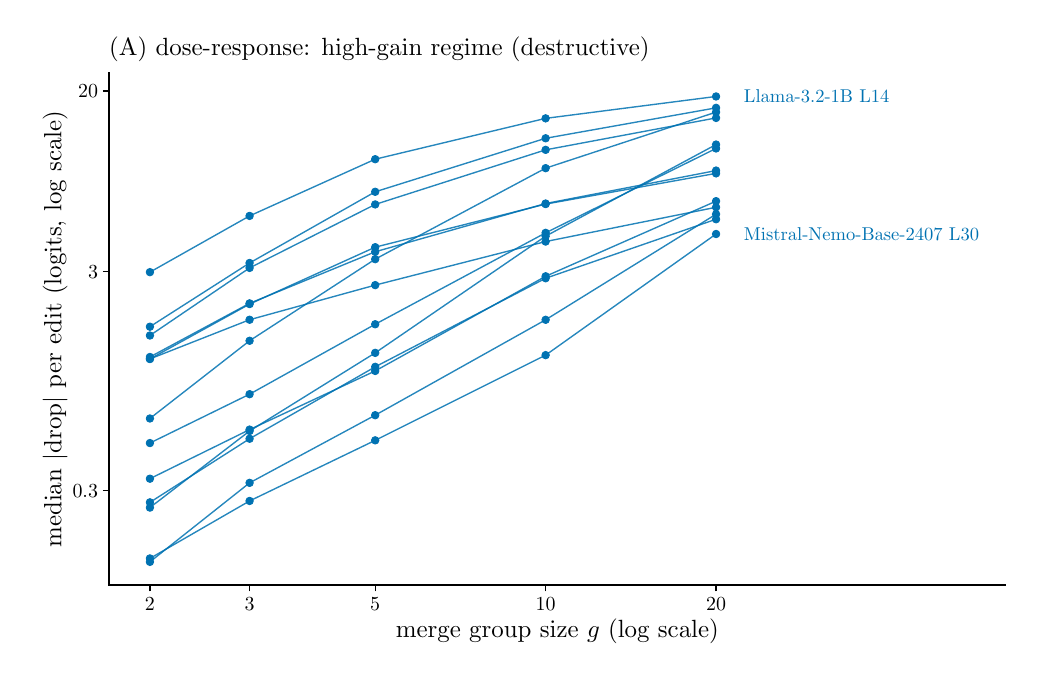
\begin{tikzpicture}[x=1pt,y=1pt]
\definecolor{fillColor}{RGB}{255,255,255}
\path[use as bounding box,fill=fillColor,fill opacity=0.00] (0,0) rectangle (361.35,224.04);
\begin{scope}
\path[clip] (  0.00,  0.00) rectangle (361.35,224.04);
\definecolor{drawColor}{RGB}{255,255,255}
\definecolor{fillColor}{RGB}{255,255,255}

\path[draw=drawColor,line width= 0.5pt,line join=round,line cap=round,fill=fillColor] (  0.00,  0.00) rectangle (361.35,224.04);
\end{scope}
\begin{scope}
\path[clip] ( 29.45, 22.61) rectangle (353.35,207.59);
\definecolor{fillColor}{RGB}{255,255,255}

\path[fill=fillColor] ( 29.45, 22.61) rectangle (353.35,207.59);
\definecolor{drawColor}{RGB}{0,114,178}

\path[draw=drawColor,draw opacity=0.85,line width= 0.5pt,line join=round] ( 44.17,104.34) --
	( 80.19,118.50) --
	(125.58,131.01) --
	(187.16,146.75) --
	(248.75,159.14);

\path[draw=drawColor,draw opacity=0.85,line width= 0.5pt,line join=round] ( 44.17,105.04) --
	( 80.19,124.42) --
	(125.58,143.06) --
	(187.16,160.49) --
	(248.75,172.40);

\path[draw=drawColor,draw opacity=0.85,line width= 0.5pt,line join=round] ( 44.17,104.33) --
	( 80.19,124.16) --
	(125.58,144.72) --
	(187.16,160.29) --
	(248.75,171.39);

\path[draw=drawColor,draw opacity=0.85,line width= 0.5pt,line join=round] ( 44.17, 50.62) --
	( 80.19, 78.30) --
	(125.58,106.53) --
	(187.16,148.70) --
	(248.75,181.80);

\path[draw=drawColor,draw opacity=0.85,line width= 0.5pt,line join=round] ( 44.17,115.98) --
	( 80.19,139.01) --
	(125.58,164.73) --
	(187.16,184.07) --
	(248.75,195.06);

\path[draw=drawColor,draw opacity=0.85,line width= 0.5pt,line join=round] ( 44.17,135.70) --
	( 80.19,156.02) --
	(125.58,176.51) --
	(187.16,191.27) --
	(248.75,199.18);

\path[draw=drawColor,draw opacity=0.85,line width= 0.5pt,line join=round] ( 44.17,112.80) --
	( 80.19,137.23) --
	(125.58,160.17) --
	(187.16,179.89) --
	(248.75,191.42);

\path[draw=drawColor,draw opacity=0.85,line width= 0.5pt,line join=round] ( 44.17, 82.82) --
	( 80.19,110.90) --
	(125.58,140.39) --
	(187.16,173.27) --
	(248.75,193.52);

\path[draw=drawColor,draw opacity=0.85,line width= 0.5pt,line join=round] ( 44.17, 31.01) --
	( 80.19, 59.56) --
	(125.58, 84.01) --
	(187.16,118.48) --
	(248.75,156.64);

\path[draw=drawColor,draw opacity=0.85,line width= 0.5pt,line join=round] ( 44.17, 32.25) --
	( 80.19, 53.02) --
	(125.58, 74.92) --
	(187.16,105.71) --
	(248.75,149.48);

\path[draw=drawColor,draw opacity=0.85,line width= 0.5pt,line join=round] ( 44.17, 52.51) --
	( 80.19, 75.50) --
	(125.58,101.48) --
	(187.16,133.49) --
	(248.75,154.82);

\path[draw=drawColor,draw opacity=0.85,line width= 0.5pt,line join=round] ( 44.17, 73.94) --
	( 80.19, 91.60) --
	(125.58,116.87) --
	(187.16,149.90) --
	(248.75,180.39);

\path[draw=drawColor,draw opacity=0.85,line width= 0.5pt,line join=round] ( 44.17, 61.06) --
	( 80.19, 78.80) --
	(125.58,100.00) --
	(187.16,134.20) --
	(248.75,161.35);
\definecolor{drawColor}{RGB}{0,114,178}
\definecolor{fillColor}{RGB}{0,114,178}

\path[draw=drawColor,line width= 0.3pt,line join=round,line cap=round,fill=fillColor] ( 44.17, 50.62) circle (  1.36);

\path[draw=drawColor,line width= 0.3pt,line join=round,line cap=round,fill=fillColor] ( 80.19, 78.30) circle (  1.36);

\path[draw=drawColor,line width= 0.3pt,line join=round,line cap=round,fill=fillColor] (125.58,106.53) circle (  1.36);

\path[draw=drawColor,line width= 0.3pt,line join=round,line cap=round,fill=fillColor] (187.16,148.70) circle (  1.36);

\path[draw=drawColor,line width= 0.3pt,line join=round,line cap=round,fill=fillColor] (248.75,181.80) circle (  1.36);

\path[draw=drawColor,line width= 0.3pt,line join=round,line cap=round,fill=fillColor] ( 44.17,115.98) circle (  1.36);

\path[draw=drawColor,line width= 0.3pt,line join=round,line cap=round,fill=fillColor] ( 80.19,139.01) circle (  1.36);

\path[draw=drawColor,line width= 0.3pt,line join=round,line cap=round,fill=fillColor] (125.58,164.73) circle (  1.36);

\path[draw=drawColor,line width= 0.3pt,line join=round,line cap=round,fill=fillColor] (187.16,184.07) circle (  1.36);

\path[draw=drawColor,line width= 0.3pt,line join=round,line cap=round,fill=fillColor] (248.75,195.06) circle (  1.36);

\path[draw=drawColor,line width= 0.3pt,line join=round,line cap=round,fill=fillColor] ( 44.17,135.70) circle (  1.36);

\path[draw=drawColor,line width= 0.3pt,line join=round,line cap=round,fill=fillColor] ( 80.19,156.02) circle (  1.36);

\path[draw=drawColor,line width= 0.3pt,line join=round,line cap=round,fill=fillColor] (125.58,176.51) circle (  1.36);

\path[draw=drawColor,line width= 0.3pt,line join=round,line cap=round,fill=fillColor] (187.16,191.27) circle (  1.36);

\path[draw=drawColor,line width= 0.3pt,line join=round,line cap=round,fill=fillColor] (248.75,199.18) circle (  1.36);

\path[draw=drawColor,line width= 0.3pt,line join=round,line cap=round,fill=fillColor] ( 44.17,112.80) circle (  1.36);

\path[draw=drawColor,line width= 0.3pt,line join=round,line cap=round,fill=fillColor] ( 80.19,137.23) circle (  1.36);

\path[draw=drawColor,line width= 0.3pt,line join=round,line cap=round,fill=fillColor] (125.58,160.17) circle (  1.36);

\path[draw=drawColor,line width= 0.3pt,line join=round,line cap=round,fill=fillColor] (187.16,179.89) circle (  1.36);

\path[draw=drawColor,line width= 0.3pt,line join=round,line cap=round,fill=fillColor] (248.75,191.42) circle (  1.36);

\path[draw=drawColor,line width= 0.3pt,line join=round,line cap=round,fill=fillColor] ( 44.17, 82.82) circle (  1.36);

\path[draw=drawColor,line width= 0.3pt,line join=round,line cap=round,fill=fillColor] ( 80.19,110.90) circle (  1.36);

\path[draw=drawColor,line width= 0.3pt,line join=round,line cap=round,fill=fillColor] (125.58,140.39) circle (  1.36);

\path[draw=drawColor,line width= 0.3pt,line join=round,line cap=round,fill=fillColor] (187.16,173.27) circle (  1.36);

\path[draw=drawColor,line width= 0.3pt,line join=round,line cap=round,fill=fillColor] (248.75,193.52) circle (  1.36);

\path[draw=drawColor,line width= 0.3pt,line join=round,line cap=round,fill=fillColor] ( 44.17, 31.01) circle (  1.36);

\path[draw=drawColor,line width= 0.3pt,line join=round,line cap=round,fill=fillColor] ( 80.19, 59.56) circle (  1.36);

\path[draw=drawColor,line width= 0.3pt,line join=round,line cap=round,fill=fillColor] (125.58, 84.01) circle (  1.36);

\path[draw=drawColor,line width= 0.3pt,line join=round,line cap=round,fill=fillColor] (187.16,118.48) circle (  1.36);

\path[draw=drawColor,line width= 0.3pt,line join=round,line cap=round,fill=fillColor] (248.75,156.64) circle (  1.36);

\path[draw=drawColor,line width= 0.3pt,line join=round,line cap=round,fill=fillColor] ( 44.17, 32.25) circle (  1.36);

\path[draw=drawColor,line width= 0.3pt,line join=round,line cap=round,fill=fillColor] ( 80.19, 53.02) circle (  1.36);

\path[draw=drawColor,line width= 0.3pt,line join=round,line cap=round,fill=fillColor] (125.58, 74.92) circle (  1.36);

\path[draw=drawColor,line width= 0.3pt,line join=round,line cap=round,fill=fillColor] (187.16,105.71) circle (  1.36);

\path[draw=drawColor,line width= 0.3pt,line join=round,line cap=round,fill=fillColor] (248.75,149.48) circle (  1.36);

\path[draw=drawColor,line width= 0.3pt,line join=round,line cap=round,fill=fillColor] ( 44.17, 52.51) circle (  1.36);

\path[draw=drawColor,line width= 0.3pt,line join=round,line cap=round,fill=fillColor] ( 80.19, 75.50) circle (  1.36);

\path[draw=drawColor,line width= 0.3pt,line join=round,line cap=round,fill=fillColor] (125.58,101.48) circle (  1.36);

\path[draw=drawColor,line width= 0.3pt,line join=round,line cap=round,fill=fillColor] (187.16,133.49) circle (  1.36);

\path[draw=drawColor,line width= 0.3pt,line join=round,line cap=round,fill=fillColor] (248.75,154.82) circle (  1.36);

\path[draw=drawColor,line width= 0.3pt,line join=round,line cap=round,fill=fillColor] ( 44.17, 73.94) circle (  1.36);

\path[draw=drawColor,line width= 0.3pt,line join=round,line cap=round,fill=fillColor] ( 80.19, 91.60) circle (  1.36);

\path[draw=drawColor,line width= 0.3pt,line join=round,line cap=round,fill=fillColor] (125.58,116.87) circle (  1.36);

\path[draw=drawColor,line width= 0.3pt,line join=round,line cap=round,fill=fillColor] (187.16,149.90) circle (  1.36);

\path[draw=drawColor,line width= 0.3pt,line join=round,line cap=round,fill=fillColor] (248.75,180.39) circle (  1.36);

\path[draw=drawColor,line width= 0.3pt,line join=round,line cap=round,fill=fillColor] ( 44.17, 61.06) circle (  1.36);

\path[draw=drawColor,line width= 0.3pt,line join=round,line cap=round,fill=fillColor] ( 80.19, 78.80) circle (  1.36);

\path[draw=drawColor,line width= 0.3pt,line join=round,line cap=round,fill=fillColor] (125.58,100.00) circle (  1.36);

\path[draw=drawColor,line width= 0.3pt,line join=round,line cap=round,fill=fillColor] (187.16,134.20) circle (  1.36);

\path[draw=drawColor,line width= 0.3pt,line join=round,line cap=round,fill=fillColor] (248.75,161.35) circle (  1.36);

\path[draw=drawColor,line width= 0.3pt,line join=round,line cap=round,fill=fillColor] ( 44.17,104.34) circle (  1.36);

\path[draw=drawColor,line width= 0.3pt,line join=round,line cap=round,fill=fillColor] ( 80.19,118.50) circle (  1.36);

\path[draw=drawColor,line width= 0.3pt,line join=round,line cap=round,fill=fillColor] (125.58,131.01) circle (  1.36);

\path[draw=drawColor,line width= 0.3pt,line join=round,line cap=round,fill=fillColor] (187.16,146.75) circle (  1.36);

\path[draw=drawColor,line width= 0.3pt,line join=round,line cap=round,fill=fillColor] (248.75,159.14) circle (  1.36);

\path[draw=drawColor,line width= 0.3pt,line join=round,line cap=round,fill=fillColor] ( 44.17,105.04) circle (  1.36);

\path[draw=drawColor,line width= 0.3pt,line join=round,line cap=round,fill=fillColor] ( 80.19,124.42) circle (  1.36);

\path[draw=drawColor,line width= 0.3pt,line join=round,line cap=round,fill=fillColor] (125.58,143.06) circle (  1.36);

\path[draw=drawColor,line width= 0.3pt,line join=round,line cap=round,fill=fillColor] (187.16,160.49) circle (  1.36);

\path[draw=drawColor,line width= 0.3pt,line join=round,line cap=round,fill=fillColor] (248.75,172.40) circle (  1.36);

\path[draw=drawColor,line width= 0.3pt,line join=round,line cap=round,fill=fillColor] ( 44.17,104.33) circle (  1.36);

\path[draw=drawColor,line width= 0.3pt,line join=round,line cap=round,fill=fillColor] ( 80.19,124.16) circle (  1.36);

\path[draw=drawColor,line width= 0.3pt,line join=round,line cap=round,fill=fillColor] (125.58,144.72) circle (  1.36);

\path[draw=drawColor,line width= 0.3pt,line join=round,line cap=round,fill=fillColor] (187.16,160.29) circle (  1.36);

\path[draw=drawColor,line width= 0.3pt,line join=round,line cap=round,fill=fillColor] (248.75,171.39) circle (  1.36);

\node[text=drawColor,anchor=base west,inner sep=0pt, outer sep=0pt, scale=  0.67] at (258.82,196.88) {Llama-3.2-1B L14};

\node[text=drawColor,anchor=base west,inner sep=0pt, outer sep=0pt, scale=  0.67] at (258.82,147.18) {Mistral-Nemo-Base-2407 L30};
\end{scope}
\begin{scope}
\path[clip] (  0.00,  0.00) rectangle (361.35,224.04);
\definecolor{drawColor}{RGB}{0,0,0}

\path[draw=drawColor,line width= 0.5pt,line join=round,line cap=rect] ( 29.45, 22.61) --
	( 29.45,207.59);
\end{scope}
\begin{scope}
\path[clip] (  0.00,  0.00) rectangle (361.35,224.04);
\definecolor{drawColor}{RGB}{0,0,0}

\node[text=drawColor,anchor=base east,inner sep=0pt, outer sep=0pt, scale=  0.72] at ( 25.40, 54.31) {0.3};

\node[text=drawColor,anchor=base east,inner sep=0pt, outer sep=0pt, scale=  0.72] at ( 25.40,133.43) {3};

\node[text=drawColor,anchor=base east,inner sep=0pt, outer sep=0pt, scale=  0.72] at ( 25.40,198.63) {20};
\end{scope}
\begin{scope}
\path[clip] (  0.00,  0.00) rectangle (361.35,224.04);
\definecolor{drawColor}{RGB}{0,0,0}

\path[draw=drawColor,line width= 0.5pt,line join=round] ( 27.20, 56.79) --
	( 29.45, 56.79);

\path[draw=drawColor,line width= 0.5pt,line join=round] ( 27.20,135.91) --
	( 29.45,135.91);

\path[draw=drawColor,line width= 0.5pt,line join=round] ( 27.20,201.11) --
	( 29.45,201.11);
\end{scope}
\begin{scope}
\path[clip] (  0.00,  0.00) rectangle (361.35,224.04);
\definecolor{drawColor}{RGB}{0,0,0}

\path[draw=drawColor,line width= 0.5pt,line join=round,line cap=rect] ( 29.45, 22.61) --
	(353.35, 22.61);
\end{scope}
\begin{scope}
\path[clip] (  0.00,  0.00) rectangle (361.35,224.04);
\definecolor{drawColor}{RGB}{0,0,0}

\path[draw=drawColor,line width= 0.5pt,line join=round] ( 44.17, 20.36) --
	( 44.17, 22.61);

\path[draw=drawColor,line width= 0.5pt,line join=round] ( 80.19, 20.36) --
	( 80.19, 22.61);

\path[draw=drawColor,line width= 0.5pt,line join=round] (125.58, 20.36) --
	(125.58, 22.61);

\path[draw=drawColor,line width= 0.5pt,line join=round] (187.16, 20.36) --
	(187.16, 22.61);

\path[draw=drawColor,line width= 0.5pt,line join=round] (248.75, 20.36) --
	(248.75, 22.61);
\end{scope}
\begin{scope}
\path[clip] (  0.00,  0.00) rectangle (361.35,224.04);
\definecolor{drawColor}{RGB}{0,0,0}

\node[text=drawColor,anchor=base,inner sep=0pt, outer sep=0pt, scale=  0.72] at ( 44.17, 13.60) {2};

\node[text=drawColor,anchor=base,inner sep=0pt, outer sep=0pt, scale=  0.72] at ( 80.19, 13.60) {3};

\node[text=drawColor,anchor=base,inner sep=0pt, outer sep=0pt, scale=  0.72] at (125.58, 13.60) {5};

\node[text=drawColor,anchor=base,inner sep=0pt, outer sep=0pt, scale=  0.72] at (187.16, 13.60) {10};

\node[text=drawColor,anchor=base,inner sep=0pt, outer sep=0pt, scale=  0.72] at (248.75, 13.60) {20};
\end{scope}
\begin{scope}
\path[clip] (  0.00,  0.00) rectangle (361.35,224.04);
\definecolor{drawColor}{RGB}{0,0,0}

\node[text=drawColor,anchor=base,inner sep=0pt, outer sep=0pt, scale=  0.90] at (191.40,  3.75) {merge group size $g$ (log scale)};
\end{scope}
\begin{scope}
\path[clip] (  0.00,  0.00) rectangle (361.35,224.04);
\definecolor{drawColor}{RGB}{0,0,0}

\node[text=drawColor,rotate= 90.00,anchor=base,inner sep=0pt, outer sep=0pt, scale=  0.90] at ( 12.20,115.10) {median $|$drop$|$ per edit (logits, log scale)};
\end{scope}
\begin{scope}
\path[clip] (  0.00,  0.00) rectangle (361.35,224.04);
\definecolor{drawColor}{RGB}{0,0,0}

\node[text=drawColor,anchor=base west,inner sep=0pt, outer sep=0pt, scale=  0.90] at ( 29.45,213.84) {(A) dose-response: high-gain regime (destructive)};
\end{scope}
\end{tikzpicture}
